% questions.tex —— 2003 年·全国旧课程卷·文科 · 题目内容片段（无答案）
% 由 tools/generate_projects.py 依来源总账自 2003/2003_数学真题_全国旧课程文_试题.md 生成，勿手改（改源 MD 后重跑）


\gkpart{数学}

\begin{gktip}
\textbf{来源说明}：本题面依据固定源 PDF 两页 A3 题面逐题转录，原卷印刷页码 136–137。固定源不附答案，答案和解析均由本库独立复算。

\textbf{图形说明}：第 16、17、21、22 题的原卷图形关系重绘为 TikZ/PGFPlots 矢量图。图形标记所指的 PNG 不随仓库保存。
\end{gktip}

\gkpart{一、选择题}

\begin{question}
\gkti{1}直线 $y=2x$ 关于 $x$ 轴对称的直线方程为\mbox{（　　）}

（A）$y=-\dfrac12x$　　（B）$y=\dfrac12x$　　（C）$y=-2x$　　（D）$y=2x$

\end{question}
\begin{question}
\gkti{2}已知 $x\in\left(-\dfrac\pi2,0\right)$，$\cos x=\dfrac45$，则 $\tan2x=$\mbox{（　　）}

（A）$\dfrac7{24}$　　（B）$-\dfrac7{24}$　　（C）$\dfrac{24}{7}$　　（D）$-\dfrac{24}{7}$

\end{question}
\begin{question}
\gkti{3}抛物线 $y=ax^2$ 的准线方程是 $y=2$，则 $a$ 的值为\mbox{（　　）}

（A）$\dfrac18$　　（B）$-\dfrac18$　　（C）$8$　　（D）$-8$

\end{question}
\begin{question}
\gkti{4}等差数列 $\{a_n\}$ 中，已知 $a_1=\dfrac13$，$a_2+a_5=4$，$a_n=33$，则 $n$ 为\mbox{（　　）}

（A）48　　（B）49　　（C）50　　（D）51

\end{question}
\begin{question}
\gkti{5}双曲线虚轴的一个端点为 $M$，两个焦点为 $F_1\text{、}F_2$，$\angle F_1MF_2=120^\circ$，则双曲线的离心率为\mbox{（　　）}

（A）$\sqrt3$　　（B）$\dfrac{\sqrt6}{2}$　　（C）$\dfrac{\sqrt6}{3}$　　（D）$\dfrac{\sqrt3}{3}$

\end{question}
\begin{question}
\gkti{6}设函数

\nopagebreak[4]
\[
f(x)=
\begin{cases}
2^{-x}-1,&x\leqslant0,\\
x^2,&x>0,
\end{cases}
\]

若 $f(x_0)>1$，则 $x_0$ 的取值范围是\mbox{（　　）}

（A）$(-1,1)$　　（B）$(-1,+\infty)$

（C）$(-\infty,-2)\cup(0,+\infty)$　　（D）$(-\infty,-1)\cup(1,+\infty)$

\end{question}
\begin{question}
\gkti{7}已知 $f(x^5)=\lg x$，则 $f(2)=$\mbox{（　　）}

（A）$\lg2$　　（B）$\lg32$　　（C）$\lg\dfrac1{32}$　　（D）$\dfrac15\lg2$

\end{question}
\begin{question}
\gkti{8}函数 $y=\sin(x+\varphi)$（$0\leqslant\varphi\leqslant\pi$）是 $\mathbb R$ 上的偶函数，则 $\varphi=$\mbox{（　　）}

（A）$0$　　（B）$\dfrac\pi4$　　（C）$\dfrac\pi2$　　（D）$\pi$

\end{question}
\begin{question}
\gkti{9}已知点 $(a,2)$（$a>0$）到直线 $l:x-y+3=0$ 的距离为 $1$，则 $a=$\mbox{（　　）}

（A）$\sqrt2$　　（B）$2-\sqrt2$　　（C）$\sqrt2-1$　　（D）$\sqrt2+1$

\end{question}
\begin{question}
\gkti{10}已知圆锥的底面半径为 $R$、高为 $3R$，它的内接圆柱的底面半径为 $\dfrac34R$，该圆柱的全面积为\mbox{（　　）}

（A）$2\pi R^2$　　（B）$\dfrac94\pi R^2$　　（C）$\dfrac83\pi R^2$　　（D）$\dfrac52\pi R^2$

\end{question}
\begin{question}
\gkti{11}已知长方形的四个顶点 $A(0,0)\text{、}B(2,0)\text{、}C(2,1)\text{、}D(0,1)$，一质点从 $AB$ 的中点 $P_0$ 沿与 $AB$ 的夹角为 $\theta$ 的方向射到 $BC$ 上的点 $P_1$ 后，依次反射到 $CD\text{、}DA$ 和 $AB$ 上的点 $P_2\text{、}P_3$ 和 $P_4$（入射角等于反射角）。若 $P_4$ 与 $P_0$ 重合，则 $\tan\theta=$\mbox{（　　）}

（A）$\dfrac13$　　（B）$\dfrac25$　　（C）$\dfrac12$　　（D）$1$

\end{question}
\begin{question}
\gkti{12}一个四面体的所有棱长都为 $\sqrt2$，四个顶点在同一球面上，则此球的表面积为\mbox{（　　）}

（A）$3\pi$　　（B）$4\pi$　　（C）$3\sqrt3\pi$　　（D）$6\pi$

\end{question}
\gkpart{二、填空题}

\begin{question}
\gkti{13}不等式 $\sqrt{4x-x^2}<x$ 的解集是\gkblank{}。

\end{question}
\begin{question}
\gkti{14}$\left(x^2-\dfrac1{2x}\right)^9$ 的展开式中 $x^9$ 的系数是\gkblank{}。

\end{question}
\begin{question}
\gkti{15}在平面几何里，有勾股定理：“设 $\triangle ABC$ 的两边 $AB\text{、}AC$ 互相垂直，则 $AB^2+AC^2=BC^2$。”拓展到空间，类比平面几何的勾股定理，研究三棱锥的侧面面积与底面面积间的关系，可以得出的正确结论是：“设三棱锥 $A-BCD$ 的三个侧面 $ABC\text{、}ACD\text{、}ADB$ 两两互相垂直，则\gkblank{}。”

\Needspace{0.4\textheight}
\end{question}
\begin{question}
\gkti{16}如图，一个地区分为 5 个行政区域，现给地图着色，要求相邻地区不得使用同一颜色，现有 4 种颜色可供选择，则不同的着色方法共有\gkblank{}种。（以数字作答）
\nopagebreak[4]
\begin{center}% 2003 年全国旧课程文科第 16 题：行政区域着色图
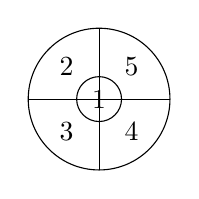
\begin{tikzpicture}[scale=0.75]
  \draw (0,0) circle (1.2);
  \draw (0,-1.2)--(0,1.2) (-1.2,0)--(1.2,0);
  \draw (0,0) circle (0.38);
  \node at (0,0) {1};
  \node at (-0.55,0.55) {2};
  \node at (0.55,0.55) {5};
  \node at (-0.55,-0.55) {3};
  \node at (0.55,-0.55) {4};
\end{tikzpicture}
\end{center}
\nopagebreak[4]
\end{question}
\gkpart{三、解答题}

\Needspace{0.4\textheight}
\begin{question}
\gkti{17}已知正四棱柱 $ABCD-A_1B_1C_1D_1$，$AB=1$，$AA_1=2$，$E$ 为 $CC_1$ 中点，$F$ 为 $BD_1$ 中点。
\nopagebreak[4]
\begin{center}% 2003 年全国旧课程文科第 17 题：正四棱柱
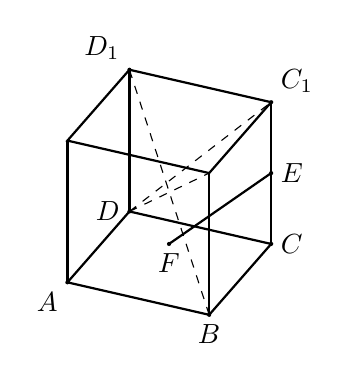
\begin{tikzpicture}[>=stealth,scale=0.75]
  \coordinate (A) at (0,0); \coordinate (B) at (2.4,-0.55);
  \coordinate (C) at (3.45,0.65); \coordinate (D) at (1.05,1.2);
  \coordinate (A1) at (0,2.4); \coordinate (B1) at (2.4,1.85);
  \coordinate (C1) at (3.45,3.05); \coordinate (D1) at (1.05,3.6);
  \coordinate (E) at (3.45,1.85); \coordinate (F) at (1.72,0.65);
  \draw[thick] (A)--(B)--(C)--(D)--cycle;
  \draw[thick] (A1)--(B1)--(C1)--(D1)--cycle;
  \draw[thick] (A)--(A1) (B)--(B1) (C)--(C1) (D)--(D1);
  \draw[dashed] (B)--(D1) (D)--(B1) (D)--(C1);
  \draw[thick] (E)--(F);
  \fill (A) circle (1pt) node[below left] {$A$};
  \fill (B) circle (1pt) node[below] {$B$};
  \fill (C) circle (1pt) node[right] {$C$};
  \fill (D) circle (1pt) node[left] {$D$};
  \fill (D1) circle (1pt) node[above left] {$D_1$};
  \fill (C1) circle (1pt) node[above right] {$C_1$};
  \fill (E) circle (1pt) node[right] {$E$};
  \fill (F) circle (1pt) node[below] {$F$};
\end{tikzpicture}
\end{center}
\nopagebreak[4]
（1） 证明：$EF$ 为 $BD_1$ 与 $CC_1$ 的公垂线；

（2） 求点 $D_1$ 到面 $BDE$ 的距离。

\end{question}
\begin{question}
\gkti{18}已知复数 $z$ 的辐角为 $60^\circ$，且 $|z-1|$ 是 $|z|$ 和 $|z-2|$ 的等比中项，求 $|z|$。

\end{question}
\begin{question}
\gkti{19}已知数列 $\{a_n\}$ 满足 $a_1=1$，$a_n=3^{n-1}+a_{n-1}$（$n\geqslant2$）。

（1） 求 $a_2\text{、}a_3$；

（2） 证明：$a_n=\dfrac{3^n-1}{2}$。

\Needspace{0.4\textheight}
\end{question}
\begin{question}
\gkti{20}已知函数

\nopagebreak[4]
\[
f(x)=2\sin x(\sin x+\cos x).
\]

（1） 求函数 $f(x)$ 的最小正周期和最大值；

（2） 在给出的直角坐标系中，画出函数 $y=f(x)$ 在区间 $\left[-\dfrac\pi2,\dfrac\pi2\right]$ 上的图象。
\nopagebreak[4]
\begin{center}% 2003 年全国旧课程文科第 20 题：函数图象坐标系
\begin{tikzpicture}[x=1.0cm,y=0.7cm,>=stealth]
  \draw[->] (-1.9,0)--(1.9,0) node[right] {$x$};
  \draw[->] (0,-1.4)--(0,1.6) node[above] {$y$};
  \node[below] at (-1.57,0) {$-\frac\pi2$};
  \node[below] at (1.57,0) {$\frac\pi2$};
  \node[below left] at (0,0) {$O$};
\end{tikzpicture}
\end{center}
\nopagebreak[4]
\Needspace{0.4\textheight}
\end{question}
\begin{question}
\gkti{21}在某海滨城市附近海面有一台风。据监测，当前台风中心位于城市 $O$（如图）的东偏南 $\theta$ 方向 300 km 的海面 $P$ 处，并以 20 km/h 的速度向西偏北 $45^\circ$ 方向移动，台风侵袭的范围为圆形区域，当前半径为 60 km，并以 10 km/h 的速度不断增大，问几小时后该城市开始受到台风的侵袭？
\nopagebreak[4]
\begin{center}% 2003 年全国旧课程文科第 21 题：台风运动示意图
\begin{tikzpicture}[>=stealth,scale=0.72]
  \draw[->] (-2.8,0)--(3.2,0) node[right] {东};
  \draw[->] (0,-2.3)--(0,2.5) node[above] {北};
  \fill (0,0) circle (1.5pt) node[below left] {$O$};
  \fill (-1.8,-1.25) circle (1.5pt) node[below] {$P$};
  \draw[->,thick] (-1.8,-1.25)--(0.2,0.75) node[midway,below] {$20$ km/h};
  \draw[dashed] (-1.8,-1.25) circle (0.55);
  \node at (-1.35,-1.75) {$r(t)$};
  \draw[->] (0.35,0.1) arc[start angle=15,end angle=210,radius=0.35];
\end{tikzpicture}
\end{center}
\nopagebreak[4]
\Needspace{0.4\textheight}
\end{question}
\begin{question}
\gkti{22}已知常数 $a>0$，在矩形 $ABCD$ 中，$AB=4$，$BC=4a$，$O$ 为 $AB$ 的中点，点 $E\text{、}F\text{、}G$ 分别在 $BC\text{、}CD\text{、}DA$ 上移动，且

\nopagebreak[4]
\[
\frac{BE}{BC}=\frac{CF}{CD}=\frac{DG}{DA},
\]

$P$ 为 $GE$ 与 $OF$ 的交点（如图）。问是否存在两个定点，使 $P$ 到这两点的距离之和为定值？若存在，求出这两点的坐标及此定值；若不存在，请说明理由。
\nopagebreak[4]
\begin{center}% 2003 年全国旧课程文科第 22 题：矩形动点示意图
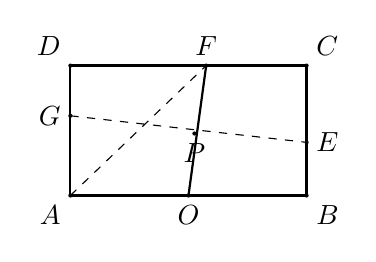
\begin{tikzpicture}[>=stealth,scale=0.75]
  \coordinate (A) at (0,0); \coordinate (B) at (4,0);
  \coordinate (C) at (4,2.2); \coordinate (D) at (0,2.2);
  \coordinate (E) at (4,0.9); \coordinate (F) at (2.3,2.2);
  \coordinate (G) at (0,1.35); \coordinate (P) at (2.1,1.05);
  \coordinate (O) at (2,0);
  \draw[thick] (A)--(B)--(C)--(D)--cycle;
  \draw[dashed] (G)--(E) (A)--(F);
  \draw[thick] (O)--(F);
  \fill (A) circle (1pt) node[below left] {$A$};
  \fill (B) circle (1pt) node[below right] {$B$};
  \fill (C) circle (1pt) node[above right] {$C$};
  \fill (D) circle (1pt) node[above left] {$D$};
  \fill (E) circle (1pt) node[right] {$E$};
  \fill (F) circle (1pt) node[above] {$F$};
  \fill (G) circle (1pt) node[left] {$G$};
  \fill (P) circle (1pt) node[below] {$P$};
  \fill (O) circle (1pt) node[below] {$O$};
\end{tikzpicture}
\end{center}
\nopagebreak[4]

\end{question}